Tämä luku sisältää kuvausta kurssin alkupuolelta, jossa ympäristöt asennettiin
toimiviksi kurssin suorittamista varten. Monet asioista ovat jo ennestään
tuttuja ja puoliksi aiemmin tehtyjä, joten osa vaiheista voi vaikuttaa tämän
seurauksena vajaalta.

\section{Rauta}

Kehitys tapahtuu lähtökohtaisesti itsekootulla pöytätietokoneella, josta
löytyy seuraavat speksit:
\begin{itemize}
    \item Suoritin: 12th Gen Intel(R) Core(TM) i7-12700K
    \item RAM: 64Gt (DDR4)
    \item Näytönohjaimet: NVIDIA GeForce GTC 1660 SUPER ja 1050 Ti
    \item Käyttöjärjestelmä: Windows 11 Pro N, 64-bittinen
\end{itemize}

Pöytäkoneen lisäksi käytössä vanha Thinkpad E540 mikäli tarvitsee tehdä asioita
muualla kuin kotona. Puhelimina käytössä uusi Google Pixel 6A (Android 13) ja
muutaman vuoden vanha Honor 8 (Android 8). Tarvittaessa laatikon pohjalta
pitäisi löytyä vanha Samsung S3 Mini (Android 4.X ?).

\section{Versionhallinta}

Kurssin puolesta versionhallinnassa käytetään Gitlabia. Luotuun repositoryyn
ei kuitenkaan ole mahdollista muokata asetuksia, joka aiheuttaa rajoitteen
ominaisuuksista, jotka edistäisivät kurssin suoritusta.

Näistä käytännössä ainut merkittävä on runnerin puuttuminen, jotta saisi
käytettyä Gitlab CI:tä oppimispäiväkirjan PDF:n luonnissa ja projektin
mahdollisten testien ja lintterin ajamiseen sekä buildaamiseen ja julkaisuun.
Runneria on mahdollista ajaa itse, mutta asetuksista tulisi rekisteröidä
käytettävä runneri. Vaihtoehtoisesti voisi käyttää jaettuja runnereita, mutta
allekirjoittaneen tämän hetken tiedon mukaan niitä ei ole eikä niistä ole mitään
kirjoitettu ohjeissa \parencite{TuniIntraGitlab}.

Runnerin puuttumisen vuoksi osa repositoryn sisällöstä (oppimispäiväkirja ja
projekti) on Githubissa julkisina repositoryina ja liitetty submoduleina.

\begin{lstlisting}[
    basicstyle=\small,
    label={lst:add-submodules},
    language=bash,
]
    $ git submodule add \
          git@github.com:Aikain/COMP.CS.220.git oppimispaivakirja
    $ git submodule add git@github.com:Aikain/Mafioso.git projekti
\end{lstlisting}

README:hen on lisätty ohjeet, jotka neuvovat miten repositoryn voi kloonata
submoduulien kanssa. Githubissa olevat submoduulit eivät vaadi Kurssin
opetushenkilöstöltä Github tunnuksia tms. Githubin käyttö aiheuttaa
rajoitteeksi sen, että kurssin opetushenkilöstö ei voi tehdä muutoksia
Githubissa sijaitseviin repositoryihin, mutta kurssin ohjeistuksen
perusteella sen ei pitäisi olla tarpeellista.

Toisena syynä ulkoiselle repositorylle projektin suhteen on halu pitää
projekti tallessa ja pyrkiä jatkamaan projektin kehittämistä kurssin
jälkeenkin. Tähän toki ratkaisuna olisi projektin siirtäminen kurssin
loputtua GIthubiin, mutta aiempien kurssien kokemuksen pohjalta asiat on
parempi tehdä aiemmin kuin myöhemmin.

Itselle valitettavasti turhankin tuttuun tapaan kuukausittainen huoltoilta
\parencite{TuniMaintenance2023_01} onnistui osumaan jälleen kerran siihen
hetkeen kun yritti avata Gitlabia. Katko onneksi kesti lyhyehkö aikaan.

Gitlabiin ja Githubiin on aiemmin lisätty SSH-avaimet ja GPG-avaimet. Nämä
avaimet on myös määritelty toimimaan koneella automaattisesti sen mukaan
missä projekti sijaitsee. Projektin ollessa koulu projekteissa, käytetään
automaattiseti seuraavia tietoja:
\begin{itemize}
    \item Nimi: Ville Nupponen
    \item Sähköposti: ville.nupponen@tuni.fi
    \item Allekirjoitus avain: E142FDB791613985
\end{itemize}

Projektin on tarkoitus kuitenkin olla projekti koulun ulkopuolellakin,
joten siellä käytössä henkilökohtaiset tiedot:
\begin{itemize}
    \item Nimi: Ville Nupponen
    \item Sähköposti: ville.nupponen@aika.in
    \item Allekirjoitus avain: B9C934218C333AF9
\end{itemize}

Kaikki commitit allekirjoitetaan GPG-avaimilla. Mahdollisesti kurssin edetessä
vaihtuu käyttöön SSH-avaimilla allekirjoittaminen sikäli kun olisi tarkoitus
siirtyä jossain välissä käyttämään sitä. Tämä on kuitenkin tästä kurssista
riippumaton muutos eikä muutenkaan näy kurssin suoritusten tekemisessä
mitenkään.

Gitlab ja Github osaavat vahvistaa committien allekirjoituksen kuvien
\ref{fig:gitlab-commit-verified} ja \ref{fig:github-commit-verified}
mukaisesti.

\begin{figure}[h!]
    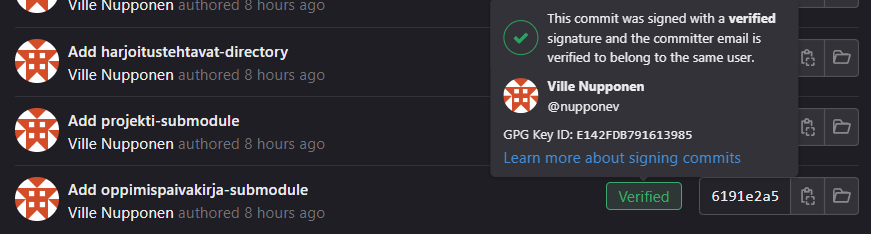
\includegraphics[width=\textwidth]{figures/gitlab-commit-verified.png}
    \caption{Kuvankaappaus Gitlabin commit listasta, jossa vahvistettu commitin allekirjoitus}
    \label{fig:gitlab-commit-verified}
\end{figure}

\begin{figure}[h!]
    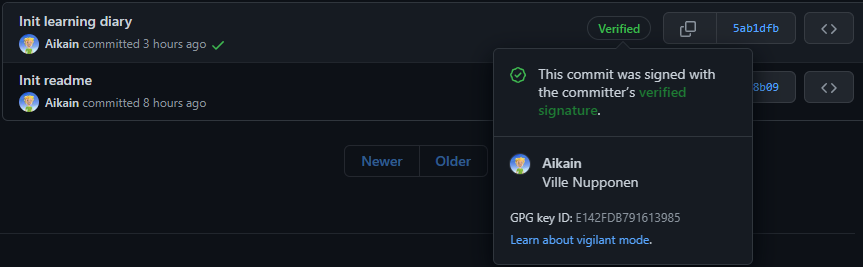
\includegraphics[width=\textwidth]{figures/github-commit-verified.png}
    \caption{Kuvankaappaus Githubin commit listasta, jossa vahvistettu commitin allekirjoitus}
    \label{fig:github-commit-verified}
\end{figure}

\section{Oppimispäiväkirja}

Oppimispäiväkirjan ohjeissa ohjeistettiin käyttämään pohjana opiskelijan
käsikirjasta löytyvää Diplomityö-ohjeessa \parencite{TuniIntraDiplomityo}
mainittua pohjaa. Ohjeista löytyy linkki Githubissa olevaan Ville Koljosen
tekemään LaTeX-pohjaan \parencite{GithubVillekolTauLatexThesisTemplate}.
Kyseinen pohja on vastaava kuin mitä käytin edellisenä vuonna kandidaationtyön
\parencite{GithubAikainCOMP200} tekemisessä.

Tämä oppimispäiväkirja on luotu kopioimalla kandidaation työn lopullinen
versio ja poistamalla kaikki sisältö. Tällöin saatiin itselle tutut asetukset
ja workflowt ilman, että tarvitsee niitä tehdä uudelleen. Pohjaa on muokattu
sen verran, että pohja ei vaadi tarkastajan kirjoittamista. Lisäksi viittaus
tapana käytetään numerointia eikä APA-merkintä tapaa. Tätä on kuitenkin
tarvittaessa helppo vaihtaa määrityksistä. Pohjassa numeeriset viittaukset
määriteltiin myös aakkosjärjestykseen kuten APA:ssa, mutta tämä johtui siitä,
ettei lähdeluettelon määrityksessä käytetty määriteltyä järjestystä.

\subsection{Kirjoittamiseen käytettävä IDE}

Kandidaatintyötä tehdessä käytössä oli Intellij IDEA ja siihen asennettuna
lisäosa, jotta saatiin tuki LaTeXille. Lisäksi koneelle asennettiin tuolloin
MiKTeX. Lisäosa ei kuitenkaan toiminut niin sujuvasti kuin olisi toivonut,
joten tällä kertaa päätin kokeilla mielestäni yksinkertaisemmalla tavalla eli
kevyemmällä IDE:llä ja terminaalilla.

Jetbrains julkaisi \parencite{JetbrainsFleetPublicPreview} 2022 lokakuussa
uuden Fleet-IDEn julkisen previewin, jonka myötä kyseistä IDEä on ollut
mahdollista käyttää ilman, että kuuluu suljettuun testiporukkaan. julkaisun
jälkeen olen itse ottanut käyttöön kaikkiin, joita varten ei selvästi ole
specifiä IDEä. Oppimispäiväkirja on pitkälti vain tekstiä, koodinpätkiä ja
kuvia, joten toimii täydellisesti siihen. Varsinaista tukea erityisesti
LaTeXille ei ole, mutta tämä ei ole merkittä muutos nähden aiempaan ratkaisuun,
jossa tuki oli hyvin olematon.

Fleet on siis jo parin kuukauden ajalta tuttu, joten se oli jo valmiina
asennettuna. Myös Fleetin navigointi ja pikanäppäimet ovat tutut ja tekevät
oppimispäiväkirjan työstämisestä LaTeXilla helpohkoa. UI on myös mukavan
minimalistinen, kuten kuvassa \ref{fig:fleet-ui} näkyy. Suurin puute on
automaattisen täytön puuttuminen, kun lisää uuden viittauksen lähteeseen,
mutta muuten ei ole aloittaessa ainakaan ilmennyt muita asioita, jotka
häiritsivät oppimispäiväkirjan tekemistä.

\begin{figure}[h!]
    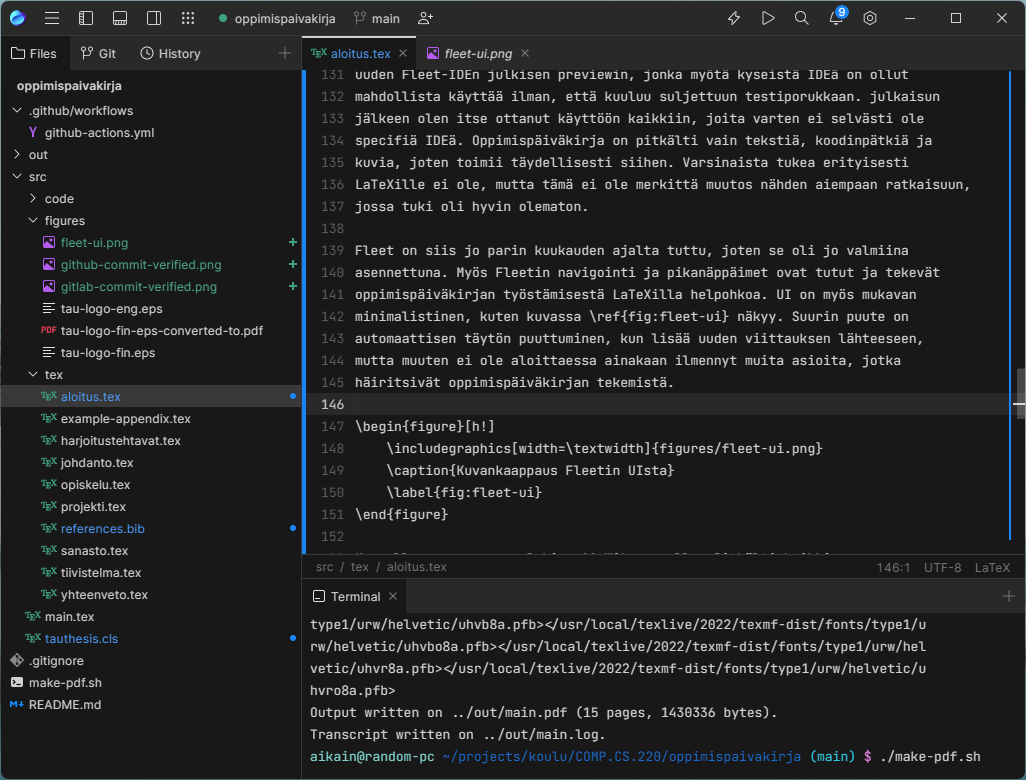
\includegraphics[width=\textwidth]{figures/fleet-ui.png}
    \caption{Kuvankaappaus Fleetin UI:sta}
    \label{fig:fleet-ui}
\end{figure}

\subsection{PDF:n generointi paikallisesti}

Koneelle on asennettu Debian 11 WSL:n avulla. Pitkälti kaikki
komentorivityökalut, joita käytän, on asennettu Debianille. Kaikki komennot,
joita tässä työssä käytetään, suoritetaan Debianin sisällä sen ollessa
luontevampaa ja kätevämpää kuin käyttää esim. cmd tai powershell. Lisäksi muut
ratkaisut, kuten cygwin, eivät ole onnistuneet osoittamaan toimivuutta yhtä
kattavasti.

Aiemmin LaTeXia käytettäessä tarvittavat ohjelmistot oli asennettu Windowsin
puolelle, joten siihen liittyvät oli nyt asennettava uudestaan. Debianin
käyttämästä pakettihallinnasta löytyi suoraan texlive-paketti, joka vaikutti
sisältävän kaiken tarvittavan, joten asennus vaikutti hyvin suoraviivaiselta:

\begin{lstlisting}[
    basicstyle=\small,
    label={lst:install-texlive},
    language=bash,
]
    # apt install texlive
\end{lstlisting}

Tämän jälkeen käytettävissä oli pdflatex-komento, jota käytetään PDF:n
generointiin. LaTeX-pohjassa löytyi valmiit ohjeet terminaali pohjaiseen
käyttöön:

\begin{lstlisting}[
    basicstyle=\small,
    label={lst:install-texlive},
    language=bash,
]
    $ pdflatex main.tex
    $ makeindex -s main.ist -t main.glg -o main.gls main.glo
    $ biber main
    $ pdflatex main.tex
    $ pdflatex main.tex
\end{lstlisting}

Kuitenkin jo ensimmäistä komentoa ajaessa ilmeni ongelmia. Komento ei
generoinut kaikkia tarvittavia tiedostoja, joita komento itse tarvitsi
myöhemmin. Lisäksi makeindex-komennon tarvitsevat main.ist- ja main.glo-
tiedosto puuttuivat. Näiden lisäksi myös biber-komentoa ei löytynyt sillä
kyseisen riippuvuutta ei saatu asennettua. pdflatex-komento varoitti lisäksi
vanhasta versioista ja ohjeisti päivittämään uuteen.

Saatuja ohjeita \parencite{TeXLiveQuickInstall} noudattaen texliven päivitys
onnistui vaivattomasti. Päivityksen jälkeen aiemmin ilmenneet ongelmat
katosivat ja ratkaistavana olivat vain yksittäiset syntaksivirheet sekä
yksi puuttuva riippuvuus. Riippuvuuksia saadaan asennettua tlmgr-komennolla.
Kyseinen komento vaatii kuitenkin ensimmäisellä kerralla alustuksen:

\begin{lstlisting}[
    basicstyle=\small,
    label={lst:init-tlmgr},
    language=bash,
]
    $ tlmgr init-usertree
\end{lstlisting}

jonka jälkeen puuttuva riippuvuus saatiin asennettua:

\begin{lstlisting}[
    basicstyle=\small,
    label={lst:init-tlmgr},
    language=bash,
]
    $ tlmgr install titlesec
\end{lstlisting}

PDF:n generointi aiemmin esiteltyhjen komentoje avulla generoi PDF:n lisäksi 16
muuta tiedostoa. Oletuksena nämä tiedostot sijoittuivat main.tex-tiedoston
kanssa samaan kansioon, joka teki oleellisista tiedostoista hankalampilöytyisiä
tiedostorakenteen kautta. Tämän seurauksena automaattisesti generoidut
tiedostot, joita ei sen myötä myöskään tarvitse lisätä versionhallintaa, olisi
kätevä saada omaan kansioonsa. Tämä onnistuu muutamalla lisäflagilla
komentoihin:

\begin{lstlisting}[
    basicstyle=\small,
    label={lst:init-tlmgr},
    language=bash,
]
    $ pdflatex -output-directory=../out main.tex
    $ biber --output-directory ../out main
\end{lstlisting}

makeindex-komento ei kuitenkaan vaikuttanut osaavan luoda tiedostoja muualla
kuin nykyiseen kansioon (tai sen alakansioihin), joten src-kansion ulkopuolella
oleva kansio ei suoraan onnistuisi. Tämä saadaan kuitenkin tehtyä vaihtamalla
kansiota kyseisen komennon ajaksi generoiduille tiedostoille luotuun kansioon.
Komentoja ollessa jo valmiiksi useita ja joiden lisäksi kansion vaihtamisia,
oli tähän kätevämpi luoda yksinkertainen bash-scripti \ref{lst:make-pdf}, joka
tekee kaiken tarvittavan.

\lstinputlisting[
    basicstyle=\small,
    caption={Bash-scripti PDF:n generointiin},
    label={lst:make-pdf},
]{code/make-pdf.sh}

Tämän jälkeen muutoksien jälkeen saadaan generoitua PDF paikallisesti:

\begin{lstlisting}[
    basicstyle=\small,
    label={lst:init-tlmgr},
    language=bash,
]
$ ~/projects/koulu/COMP.CS.220/oppimispaivakirja/make-pdf.sh
\end{lstlisting}

\subsection{PDF:n generointi automaattisesti}

Paikallisen generoinnin lisäksi PDF saadaan generoitua automaattisesti Github
Actioneiden avulla. Nämä on määritelty oppimispäiväkirjan repositoryssa
.github/workflows-kansiossa Github Action for LaTeX -actionin ohjeiden
\parencite{GithubActionsForLaTeX} mukaisesti. Määritykset saatiin suoraan
valmiiksi kopioitua kandidaationtyön repositorysta. Osasta actioneita oli
Kuitenkin tullut uudet versiot, joten ne päivitettiin uudempiin. Lisäksi
triggeröinti sääntöjä tarkennettiin, jotta PDF generoidaan vain jos sen
generointiin käytettävät tiedostot muuttuvat.

Kun muutokset commitataan ja pushataan, käynnistyy automaattisesti workflow,
joka on nähtävissä Githubissa repositoryn Actions-välilehdessä. Noin 2 minuutin
odottamisen jälkeen työ valmistuu ja ja artifakteista löytyy PDF.zip tiedosto
ladattavaksi, jonka sisältä löytyy generoitu main.pdf-tiedosto.

\subsection{Run-configuraatio Jetbrains Fleetiin}

Jetbrains Fleetiin on mahdollista määritellä Run Configuration, jonka avulla
voisi olla helpomi ajaa kuin pitää auki erillistä terminaalia, josta ajaa
komento aina eriskeen. Kuitenkaan tämän määritys ei lähtenyt toimimaan niin
yksinkertaisesti kuin olisi voinut toivoa, joten liian ajan käyttäminen ei
ole kannattavaa näin pienen asian suhteem.

\section{Android Studion asennus}

Jetbrainsin tuotteiden ollessa ennestään tuttuja ja aktiivisessa käytössä, on
käytössä myös Jetbrains Toolbox, joka mahdollistaa Jetbrainsin IDE:jen
asentamisen vaivatta. Tämän avulla onnistuu myös Android Studion asentaminen
yhdellä klikkaukselle.

Asennuksen yhteydessä ilmenee ongelma HAXM:n asentamisessa:

\begin{displayquote}
Intel® HAXM installation failed. To install Intel® HAXM follow the instructions found at: https://github.com/intel/haxm/wiki/Installation-Instructions-on-Windows
\end{displayquote}

Ongelma vaikuttaisi johtuvan Windowsin ytimen eristyksestä ja korjaantuisi se
pois kytkemällä \parencite{GithubIntelHaxmIssue412}. Kuitenkaan KAXM:n ollessa
vain parannus emulaattorin suorituskykyyn, ei ytimen eristyksen kytkeminen pois
päältä ole välttämättä kannattavaa.

Ensimmäisellä yrittämällä vaikuttaisi ettei projektin luonti toimi WSL:n
sisälle. Tähän tarkempaa perehtymistä harjoitus 3:n yhteydessä.

\section{Tuntikirjanpito}

Kurssin edetessä kirjaan tunnit niihin asioihin mihin kyseisestä asiasta
kirjoitettu teksti sisältyy oppimispäiväkirjassa. Lopullinen yhteenveto eri
osioiden yhteenlasketusta tuntikirjanpidosta löytyy yhteenvedosta.

Alla olevaan taulukkoon on kirjattu aloitukseen käytetyt tunnit. Näiden lisäksi
taulukkoon on laitettu ne tunnit, joissa on selvästi keskitytty
oppimispäiväkirjan tekemiseen niiltä osilta kun oppimispäiväkirjaa ei ole tehty
sujuvasti muun tekemisen ohessa tai on vaatinut asioiden siistiksi
kirjoittamista.

Käytetty aika on kirjattu 5min tarkkuudella. Tämä lähinnä, koska samaa käytäntöä
käyttää töissä ja helpoittaa hahmottamaan mitä asioita tehnyt ja milloin.

\begin{table}[H]
  \centering
  \label{tab:other-studing-working-hours}
  \begin{tabular*}{\linewidth}{@{\extracolsep{\fill}} l c c c r }
    \textbf{Tekeminen} & \textbf{Päivämäärä} & \textbf{Aloitettu} & \textbf{Lopetettu} & \textbf{Määrä} \\
    \hline
    Versionhallinnan alustus          & 19.01.2023 &     - &     - & 1h 00m \\
    Oppimispäiväkirjan alustus        & 19.01.2023 &     - &     - & 2h 00m \\
    Oppimispäiväkirjan kirjoittaminen & 20.01.2023 &     - &     - & 3h 00m \\
    Oppimispäiväkirjan kirjoittaminen & 23.05.2023 & 08:30 & 12:05 & 3h 35m \\
    Oppimispäiväkirjan kirjoittaminen & 29.05.2023 & 23:40 & 01:00 & 1h 20m \\
    Oppimispäiväkirjan kirjoittaminen & 30.05.2023 & 22:55 & 23:55 & 1h 00m \\
    Oppimispäiväkirjan kirjoittaminen & 31.05.2023 & 11:15 & 11:50 &    35m \\
    Oppimispäiväkirjan kirjoittaminen & 31.05.2023 & 13:00 & 13:20 &    20m \\
    Oppimispäiväkirjan kirjoittaminen & 31.05.2023 & 15:25 & 15:45 &    20m \\
    Oppimispäiväkirjan kirjoittaminen & 31.05.2023 & 22:30 & 00:15 & 1h 45m \\
    \hline
    \multicolumn{4}{l}{\textbf{Yhteensä}} & \textbf{15h 05m} \\
  \end{tabular*}
\end{table}
